
\documentclass[
	12pt,				    
	openright,			   
	oneside,			    
	a4paper,			    
    chapter=TITLE,        
    sumario=tradicional,   
	english,			  
	brazil,				   
	]{abntex2}             
 

\usepackage{newtxtext,newtxmath}
\usepackage[T1]{fontenc}		
\usepackage[utf8]{inputenc}		
\usepackage{indentfirst}		
\usepackage{graphicx}			
\usepackage{booktabs}          

\usepackage[alf,abnt-etal-text=it,abnt-emphasize=bf]{abntex2cite}	
\usepackage{tabularx}
\usepackage{multirow}
\usepackage{float}
\usepackage[portuguese,onelanguage,ruled,vlined]{algorithm2e}
\usepackage{ragged2e}
\usepackage{makecell}

\usepackage{caption}
\usepackage{etoolbox}
\captionsetup{
    justification = centering,
    singlelinecheck = false,
    labelsep = endash,
    font = bf, 
}

\usepackage{hyperref}

\floatstyle{plaintop}
\newfloat{mapa}{h!btp}{mapa}\floatname{mapa}{Mapa}
\newcommand{\mapaautorefname}{Mapa}
\newfloat{diagrama}{h!btp}{diagrama}\floatname{diagrama}{Diagrama}
\newcommand{\diagramaautorefname}{Diagrama}
\newfloat{fluxograma}{h!btp}{fluxograma}\floatname{fluxograma}{Fluxograma}
\newcommand{\fluxogramaautorefname}{Fluxograma}
\newfloat{figura}{h!btp}{figura}\floatname{figura}{Figura}
\newcommand{\figuraautorefname}{Figura}
\newfloat{quadro}{h!btp}{quadro}\floatname{quadro}{Quadro}
\newcommand{\quadroautorefname}{Quadro}
\newfloat{grafico}{h!btp}{grafico}\floatname{grafico}{Gráfico}
\newcommand{\graficoautorefname}{Gráfico}
\newfloat{tabela}{h!btp}{tabela}\floatname{tabela}{Tabela}
\newcommand{\tabelaautorefname}{Tabela}

\newenvironment{citacaodireta}{
\vspace*{8mm} \setlength{\parindent}{0cm}
\hfill \begin{minipage}{140mm}
}{
\vspace*{8mm} \end{minipage}
}


\counterwithout{equation}{chapter}


\renewcommand*{\chapnumfont}{\normalfont\bfseries\sffamily}
\renewcommand*{\chaptitlefont}{\normalfont\bfseries\sffamily}

\setsecheadstyle{\normalfont\bfseries\sffamily\upcase}
\setsubsecheadstyle{\normalfont\bfseries\sffamily\upcase}
\setsubsubsecheadstyle{\normalfont\bfseries\sffamily\upcase}
\setlength{\afterchapskip}{0.5cm}
\setlength{\aftersecskip}{0.5cm}

\setlrmarginsandblock{2,5cm}{2,5cm}{*}
\setulmarginsandblock{2,5cm}{2,5cm}{*}
\checkandfixthelayout

\setlength{\parindent}{0.75cm}

\setlength{\parskip}{0.2cm} 

\hypersetup{
        % metadonées
		pdftitle={Relatório de práticas},
		pdfauthor={IFPE},
	    pdfcreator={LaTeX with abnTeX2},
		colorlinks=true,  
    	linkcolor=black,    
    	citecolor=black,   
    	filecolor=magenta,
		urlcolor=black,     
		bookmarksdepth=4   
}
\begin{document}

\frenchspacing
\pagenumbering{gobble}

\pretextual

%\begin{titlepage}

\begin{center}

\includegraphics[width=0.2\textwidth]{figuras/Epita.png}

\resizebox{!}{0.35cm}{\textbf{Cahier des charges fonctionel et technique pour \{inserez un nom d'entreprise ici\}.}}\\

\textbf{\textit{ECOLE} EPITA}

% Identificacao da disciplina
\uppercase{\textbf{BLA BLABLA BL BLABLABLA}}

\vspace{6cm}

% Identificacao das atividades trabalhadas no relatório 
\uppercase{\textbf{BLA BLABLA BL BLABLABLABLA BLA BLABLA BLAB BLA BLABLA}}\\[5cm]


\textbf{CLERAULT Raphaël 3.2 (raphael.clerault)}

\textbf{DALOZ Léo 3.2 (leo.daloz)}

\textbf{BERTRAND Nicolas 3.2 (nicolas.bertrand)}

\textbf{CHANE Romain 3.2 (romain.chane)}

\end{center}

\vspace{0.2cm}
\hfill
\begin{minipage}{9cm}


\end{minipage}

\begin{center}
\vfill
\vspace{1cm}

CdCF \\

%Não alterar, pois coloca a mês e ano automaticamente na base da capa
\newcommand{\mes}{\ifcase\month\or 
    Janvier \or Fevrier \or Mars \or Avril \or Mai \or Juin \or 
    Juillet \or Aôut \or Septembre \or Octobre \or Novembre \or 
    Decembre \fi} 
    
\def\ano{\expandafter\YEAR\the\year}
\def\YEAR#1#2#3#4{#1#2#3#4}
    
{ \mes / \ano}


\end{center} 


\noindent\resizebox{!}{0.3cm}{\textbf{\uppercase{sommaire}}}\\
\noindent \textbf {-----------------------------------------------------------------------------------------------------------------}
\begin{itemize}
    \item \hyperref[chapter:introduction]{\uppercase{Introduction  ....................................................................................................... P.03}}
    \item \hyperref[chapter:origine]{\uppercase{Origine et nature du projet .......................................................................... P.05}}
    \item \hyperref[chapter:objet]{\uppercase{objet de l}’\uppercase{étude .................................................................................................. P.06}}
    \item \hyperref[chapter:etat]{\uppercase{état de l}'\uppercase{art .......................................................................................................... P.08}}
    \item \hyperref[chapter:entreprise]{\uppercase{Notre entreprise ................................................................................................ P.10}}
    \item \hyperref[chapter:repartition]{\uppercase{Répartition ............................................................................................................ P.11}}
    \item \hyperref[chapter:planification]{\uppercase{Avancement et planification  ..................................................................... P.12}}
    \item \hyperref[chapter:cdct]{\uppercase{Cahier des charges techniques .................................................................. P.13}}
    \item \hyperref[chapter:Conclusion]{\uppercase{Conclusion ............................................................................................................ P.15}}
\end{itemize} 

\vspace{10cm}

\begin{center}
\vfill
\vspace{0.2cm}

CdCF \\

%Não alterar, pois coloca a mês e ano automaticamente na base da capa
\newcommand{\mes}{\ifcase\month\or 
    Janvier \or Fevrier \or Mars \or Avril \or Mai \or Juin \or 
    Juillet \or Aôut \or Septembre \or Octobre \or Novembre \or 
    Decembre \fi} 
    
\def\ano{\expandafter\YEAR\the\year}
\def\YEAR#1#2#3#4{#1#2#3#4}
    
{ \mes / \ano}
\end{center} 

\gdef\clearforchapter{}

\chapter{Introduction}
\label{chapter:introduction}
A introdução é a parte inicial do texto, que contém a delimitação do assunto tratado e outros elementos necessários para apresentar o tema do relatório. É importante deixar claro na introdução as normas utilizadas para as práticas.

Todo texto que for utilizado na introdução que vier de alguma obra tais como: normas, livros, artigos e notas de aula, devem ser citadas no texto e registrado na referência bibliográfica.

Os arquivos ``\textit{main.tex}'' e ``\textit{referencias.tex}''não deve ser alterado, EXCETO se souber o que está fazendo. Quanto aos outros arquivos, há seções e avisos indicando o que pode ou não ser modificado.

Sobre parágrafos... Para dividir seu texto em parágrafos, basta apertar a tecla ``Enter'' duas vezes seguidas.

Exemplo de parágrafo.

Exemplo de parágrafo.

Exemplo de parágrafo.

Sobre os comandos... Vou descrevê-los aqui da forma mais sucinta possível. Ah, caso eu esqueça de falar, sempre lembre de colocar chaves ``\{ \}'' após os comandos. Aproveito pra dizer que é dentro dessas chaves que você vai inserir o que deseja (vai ficar mais claro assim que as explicações começarem, ou pelo menos assim penso).

Para textos em negrito, utilize o comando ``$\backslash$textbf\{\}'' colocando entre as chaves o que deseja destacar em negrito. \textbf{Exemplo de como fica um texto em negrito.}

Para textos em itálicos, utilize o comando ``$\backslash$textit\{\}'' colocando entre as chaves o que deseja destacar em itálico. \textit{Exemplo de como fica um texto em itálico.}

Para sublinhar textos, utilize o comando ``$\backslash$underline\{\}'' colocando entre as chaves o que deseja destacar. \underline{Exemplo de como fica um texto sublinhado.}

Vale destacar que você pode utilizar mais de um tipo de destaque de texto. Para isso, basta utilizar um comando dentro do outro.

\textbf{\textit{Exemplo de como fica um texto em negrito e itálico.}}

\textbf{\underline{Exemplo de como fica um texto em negrito e sublinhado.}}

\textit{\underline{Exemplo de como fica um texto em itálico e sublinhado.}}

\textbf{\textit{\underline{Exemplo de como fica um texto em negrito, itálico e sublinhado.}}}

Sobre citações... Primeiramente sugiro que dê uma olhada no arquivo ``\textit{referencias.bib}'' para que possa ver como inserir os dados bibliográficos das referências que vai utilizar e depois volte para esse trecho do texto.

Agora que já viu o arquivo mencionado no parágrafo anterior (ou pelo menos assim espero), deve ter observado que logo após o tipo de registro de bibliografia (article, misc, etc\ldots) tem um nome, tipo: ``\textit{@article\{\underline{GUEYMARD1993}}\ldots''. Esse trecho que está sublinhado é a ``\textit{label}'' da nossa citação. É a forma como podemos resgatar as informações dela sem ter que ficar digitando tudo manualmente.

Para colocar citações no início de frase, utilize o comando ``$\backslash$citeonline\{\}'' e dentro das chaves coloque a label da citação. Exemplo: \citeonline{GUEYMARD1993} exemplo exemplo exemplo exemplo exemplo, exemplo exemplo exemplo exemplo exemplo.

Para colocar citações no final de frase, utilize ``$\backslash$cite\{\}'' e dentro das chaves coloque a label da citação. Exemplo: Exemplo  exemplo exemplo exemplo exemplo exemplo, exemplo exemplo exemplo exemplo  exemplo \cite{HOVE2013}.

Citações diretas com menos de 3 linhas devem ser utilizadas aspas. Aliás, para colocar aspas, primeiro se coloca duas crases e, em seguida, duas aspas simples. Exemplo: Segundo \citeonline[p.2]{GUEYMARD1993}, ``Exemplo de citação com menos de três linhas. Exemplo de citação com menos de três linhas. Exemplo de citação com menos de três linhas.''.

Citações com mais de 3 linhas podem seguir o exemplo abaixo, que utiliza o ambiente ``$\backslash$citacao\{\}'':

\begin{citacao}
Exemplo de citação com mais de três linhas. Exemplo de citação com mais de três linhas. Exemplo de citação com mais de três linhas. Exemplo de citação com mais de três linhas. Exemplo de citação com mais de três linhas. Exemplo de citação com mais de três linhas. Exemplo de citação com mais de três linhas. \cite[p.2]{HOVE2013}
\end{citacao}

Observem que nas duas citações diretas acima consta o número da página que o trecho foi retirado. Para fazer isso, basta digitar ``[ ]'' antes da label da citação e dentro dos colchetes informar a página de onde o trecho foi extraído.

Para mais alguns comandos podem acessar a página ``\textit{Learn}'' do Overleaf clicando \href{https://pt.overleaf.com/learn}{\underline{\textit{\textbf{aqui}}}}. Nessa página tem todos os detalhes que irei colocar aqui, assim como muitos outros que não serão descritos nesse documento. \\

\chapter{Origine et nature du projet}\label{chapter:origine}

Nessa secão são descritos os objetivos da aula prática realizada. Basta falar em um parágrafo, com poucas linhas e de forma sucinta (os detalhes vem na próxima seção). E quanto aos objetivos específicos, eles são descritos na parte abaixo, utilizando o ambiente ``\textit{$\backslash$itemize\{\}}''.

Observem que a lista de objetivos específicos vai ficar em formato de tópicos. Caso fosse desejado o formato de lista numérica, poderia trocar o ``\textit{$\backslash$itemize\{\}}'' por ``\textit{$\backslash$enumerate\{\}}''.

Ou, caso deseje, pode fazer em texto corrido mesmo.

Antes que me esqueça, não precisa colocar textos após a lista de objetivos específicos. Sendo assim, pode seguir para a próxima seção.

\begin{itemize}
    \item Objetivo específico 1;
    \item Objetivo específico 2;
    \item Objetivo específico 3;
    \item Objetivo específico 4;
    \item Objetivo específico 5.
\end{itemize}

\noindent\par

 

\chapter{Objet de l’étude}\label{chapter:objet}

Nessa seção você escreve sobre a teoria, materiais utilizados, etc... Deverá abordar os materiais utilizados nas aulas práticas, bem como, os equipamentos. Por exemplo:
\begin{itemize}
    \item Material utilizado na prática: liga metálica, material compósito;
    \item Tipo de corpo de prova, geometria, dimensão;
    \item Equipamento usado para a prática: máquina de ensaio, forno, termopar, cadinho, entre outros
    \item  Parâmetros para execução da prática: temperatura de ensaio, carga utilizada, etc...
\end{itemize}

Além da abordagem sobre os materiais e equipamentos, o procedimento experimental utilizado deverá ser descrito na íntegra. E, para isso, possivelmente será necessário o uso de equações.

Em LaTeX, as equações são mais chatinhas de se fazer, mas quando pegar o jeito acaba ficando fácil. Antes da equação é interessante citar a fonte, enquanto que após a equação é interessante descrever as variáveis que a compõem.

Um exemplo de equação, apresentada no trabalho de \citeonline{andrade2016}, pode ser observada abaixo.

\begin{equation}
\frac{I_g}{I_o} = C_1^{am^{C_2}}
\label{eq:e1}
\end{equation}

Onde Ig é a irradiância glocal horizontal, Io é a irradiância extraterrestre (ambas em W/m²) e am é a massa de ar.

Observe que a estrutura do parágrafo da equação \ref{eq:e1} apresenta uma breve explicação sobre as variáveis, autor(es), etc.. Recomendo ver material na internet sobre como se escreve equações em LaTeX, visto que fazer isso por aqui ia demorar bastante. Um material que recomendo é a playlist do Prof. Dr. Ygo Neto Batista. Ensina muita coisa sobre LaTeX. Você pode acessar essa playlist clicando \href{https://www.youtube.com/playlist?list=PLXQryIxlA5TAuSzx0IhXpue_8a3htOm8v}{\underline{\textit{\textbf{aqui}}}}. Lembrando que ele utiliza alguns modelos diferentes desse para ensinar LaTeX, então alguns comandos podem servir nesse template, visto que alguns dos packages utilizados são iguais. \\

\chapter{état de l’art}\label{chapter:etat}

Os resultados deverão ser apresentados na forma de diagramas, figuras, fluxogramas, gráficos, quadros, mapas e tabelas, quando for o caso, seguida de discussão técnica e crítica sobre os mesmos. Qualquer material gráfico que não esteja na forma de tabela é designado de figura. Qualquer tabela ou figura deve ser obrigatoriamente, e previamente, citada no texto, além de ser devidamente numerada em sequência. 

%Nesse documento foram definidos os ambientes: diagrama, figura, fluxograma, gráfico, mapa, quadro e tabela.

\noindent\textbf{Figuras}

As figuras devem estar em formato EPS (caso não seja possível, pode ser JPEG ou PNG), coloridas e no tamanho que seja legível todos os detalhes. As figuras devem ser identificadas com seu número e legenda na parte inferior. Quando for o caso, identificar na figura o nome detalhes:

%Para inserir uma figura, faça o upload dela para a pasta figuras. Em seguida, podes observar e seguir o exemplo abaixo.

\begin{figura}[h!bt]
	\caption{a) associação de fontes utilizadas no experimento de eletroluminescência, b) câmera digital e c) adaptação da câmera para obtenção das imagens.}
	\begin{center}
	    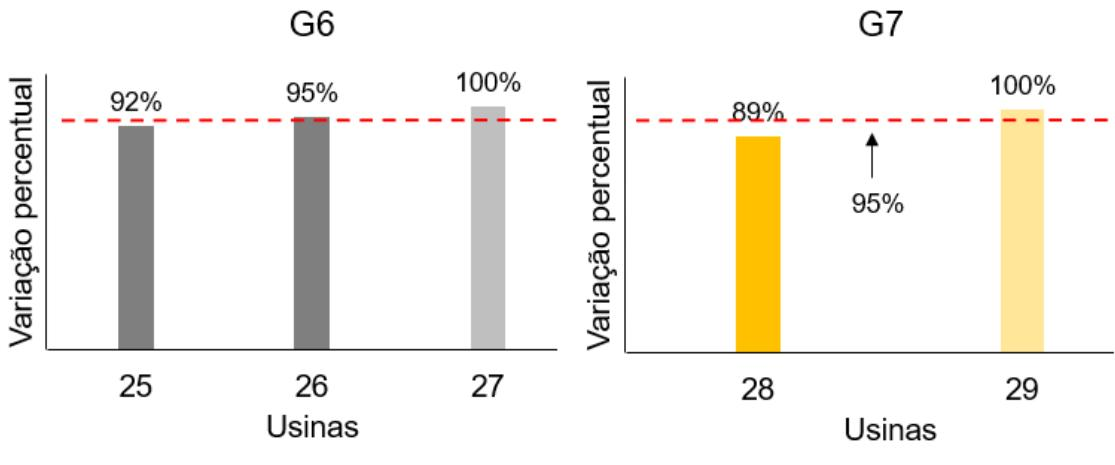
\includegraphics[scale=0.35]{figuras/fig1.jpg}
	\end{center}
    \label{grafico}
	\centering Fonte: \citeonline{FAZAL2023}
\end{figura}

Para referenciar o objeto inserido, utilize ``$\backslash$autoref\{\}''. Resultando em algo do tipo: ``Na \underline{\autoref{grafico}}, vemos que\ldots''. Caso clique no trecho sublinhado, o leitor é levado diretamente ao objeto referenciado (equação, figura, tabela, etc...).

É importante exportar imagens de boa qualidade ou em formato vetorial. Isso aumenta a qualidade da imagem no documento e permite, por exemplo, dar zoom na página sem perder o foco.

Para mais alguns comandos sobre imagens, pode acessar a página ``\textit{Como adicionar figuras em LaTeX – CL 6}'', de autoria do Felipe Cabral, clicando \href{https://vidaestudantil.com/podcasts/como-adicionar-figuras-em-latex-cl-6/}{\underline{\textit{\textbf{aqui}}}}.

\noindent \textbf{Tabelas}

As tabelas contém apenas linhas horizontais e devem estar centralizadas no documento, sendo identificada com seu número e com uma legenda na sua parte superior.

Para inserir tabela precisa de um pouco mais de dedicação. Mas vou deixar dois exemplos ``simples''.

\begin{tabela}[h!b!tp]
    \caption{Pessoas residentes em domicílios particulares, por sexo e situação do domicílio - Brasil - 1980}
    \begin{center}
        \begin{tabular}{lccc>{\centering\arraybackslash}p{1.8cm}c}
        \specialrule{2pt}{0pt}{1pt}
        \hline
        Situação do Total & Total       & Mulheres   & Homens \\
        \specialrule{1pt}{1pt}{1pt}
        Total             & 117.960.301 & 59.595.332 & 58.364.969\\
        Urbana            & 79.972.931  & 41.115.439 & 38.857.492 \\
        Rural             & 37.987.370  & 18.479.893 & 19.507.477 \\
        \specialrule{2pt}{0pt}{0pt}
        \hline
        \end{tabular}\\
    \end{center}
    \centering Fonte: IBGE (2013)
    \label{tab:Residentes}
\end{tabela}

O primeiro é uma tabela simples (\autoref{tab:Residentes}), com 4 linhas e 4 colunas. As bordas superior e inferior estão destacadas com uma espessura de linha um pouco superior em relação a linha que separa o título das demais linhas.

O segundo exemplo de tabela que vale a pena passar para vocês (e que eu passei muito tempo quebrando a cabeça para tentar fazer), é aquelas que dispões de células com quebra de texto. Vou deixar um exemplo abaixo (\autoref{tab:Comparativo dos dispositivos}) que utilizei em um dos meus trabalhos.

\begin{tabela}[h!b!tp]
    \caption{Comparação entre os dispositivos}
    \begin{center}
        \begin{tabular}{lccc>{\centering\arraybackslash}p{1.8cm}c}
        \specialrule{2pt}{0pt}{0pt}
        \hline
        Modelo & \makecell{Potência\\Ativa\\Total} & \makecell{Potência\\Reativa\\Total} & \makecell{Potência Ativa\\e Reativa\\(fundamentais)} & \makecell{Tensão e\\Corrente\\RMS} & \makecell{Variação de\\Corrente} \\
        \hline
        ADE7858A & Sim & Sim & Não & Sim & Sim \\
        ADE7868A & Sim & Sim & Não & Sim & Sim \\
        ADE7878A & Sim & Sim & Sim & Sim & Sim \\
        \specialrule{2pt}{0pt}{0pt}
        \hline
        \end{tabular}\\
    \end{center}
    \centering Fonte: Adaptado de \citeonline{ade78xxa}.
    \label{tab:Comparativo dos dispositivos}
\end{tabela}

Uma dica preciosa é que, caso ache difícil fazer as tabelas em LaTeX, pode fazer em outro software e realizar o upload para a plataforma (indico bastante o formato EPS para TODAS as imagens que forem utilizar no Overleaf). Feito isso, para identificar que se trata de uma tabela, basta seguir os comandos que constam no arquivo ``\textit{3-materiais e metodos.tex}''. %Os comandos se encontram logo abaixo desse parágrafo (mas não vão aparecer nesse PDF, então visualizem o arquivo .tex que mencionei antes). Já o resultado você pode observar na \autoref{tab:figtabela}.

\begin{tabela}[h!b!tp]
    \caption{Exemplo de tabela importada como imagem (igual a \autoref{tab:Comparativo dos dispositivos}, mas é uma imagem feita em outro software)}
    \begin{center}
        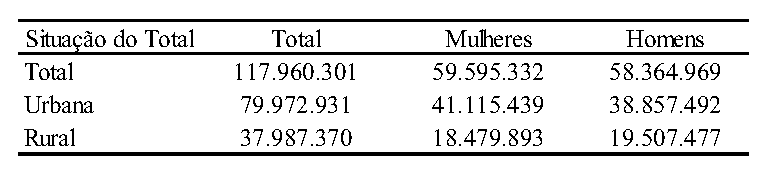
\includegraphics{figuras/figtabela.eps}
    \end{center}
    \centering Fonte: IBGE (2013)
    \label{tab:figtabela}
\end{tabela}

Certamente elementos como tamanho, formatação, letras, entre outros, da \autoref{tab:figtabela} está um pouco diferente da \autoref{tab:Residentes}. Mas a essência era mostrar que dava pra fazer a tabela em um software, mandar para um editor de imagens, exportar para o Overleaf e plotar como se fosse uma tabela (que foi exatamente o que eu fiz).

No meu caso, fiz a tabela no Excel, copiei para o CorelDRAW e exportei a imagem em formato EPS .

Mas se mesmo assim quiser fazer as tabelas aqui no Overleaf mesmo, para ensinar melhor sobre tabelas, vou indicar a página ``\textit{Como escrever tabelas em LaTeX – CL 7}'' que como sugere o título fala sobre sobre construção de tabelas em LaTeX. A página pode ser acessada clicando \href{https://vidaestudantil.com/podcasts/como-escrever-tabelas-em-latex-cl-7/}{\underline{\textit{\textbf{aqui}}}}. Também existem ferramentas online que convertem arquivos Excel parra LaTeX e/ou permitem que faça uma tabela nela própria, como por exemplo o site ``Converter Excel em LaTeX tabela'' (nome bem sugestivo) e que pode ser acessado clicando \href{https://tableconvert.com/pt/excel-to-latex}{\underline{\textit{\textbf{aqui}}}}. Para outros exemplos, basta realizar uma pesquisa rápida no Google que consegue achar vários resultados (alguns funcionais e simples, outros não).\vspace{0.2cm}

\noindent \textbf{Diagramas}

Diagrama é uma representação gráfica usada para demonstrar um esquema simplificado. Em elétrica, por exemplo, utilizamos para realizar a representação gráfica de circuitos elétricos e eletrônicos.

Abaixo tem um exemplo de diagrama.

\begin{diagrama}
    \caption{Caption}
    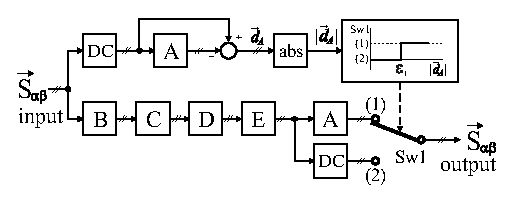
\includegraphics[width=100mm]{figuras/diagramaBlocos.eps}\\
    \centering Fonte: \citeonline{batista2015}
    \label{fig:VSGDSC}
\end{diagrama}

Eu acho que todas as dicas para apresentar esse modelo em LaTeX já foram feitas. Quaisquer outras dúvidas podem ser sanadas pelo meu \href{mailto:christian.araujo96@outlook.com}{e-mail}, Google, Bing, ChatGPT, Google Bard, YouTube, etc... \\

\chapter{Notre entreprise}\label{chapter:entreprise}
 

\newpage\chapter{Notre équipe}\label{chapter:equipe}
 

\newpage\chapter{répartition}\label{chapter:repartition}
 

\newpage\chapter{Avancement et planification}\label{chapter:planification}
 

\newpage\chapter{Cahier des charges techniques}\label{chapter:cdct}
\begin{center}
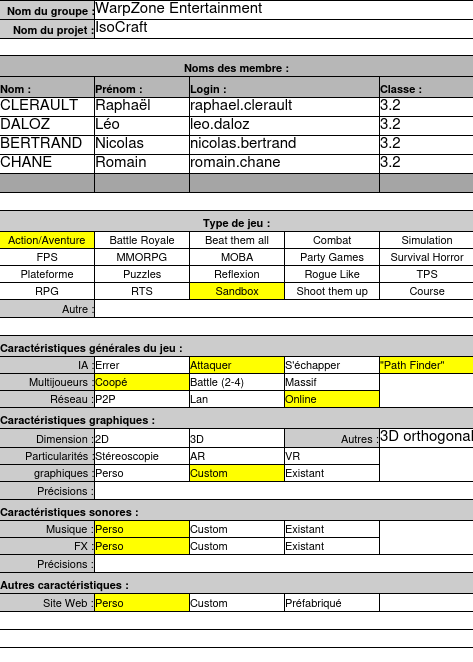
\includegraphics[width=1\textwidth]{figuras/Cahier-des-charges-technique1.png}

\newpage

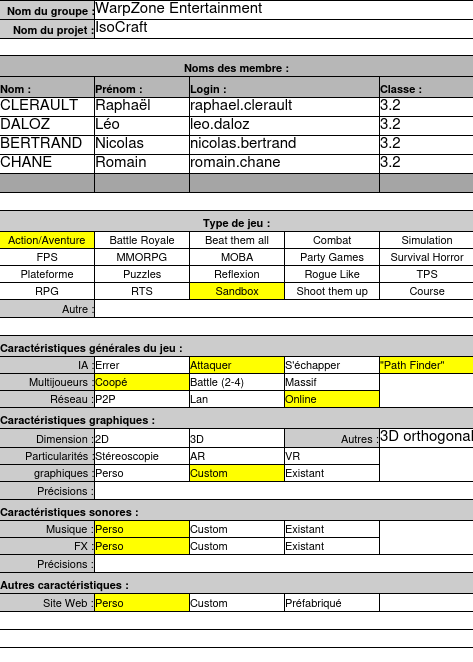
\includegraphics[width=1\textwidth]{figuras/Cahier-des-charges-technique1.png}
\end{center}

\chapter{Conclusion}\label{chapter:Conclusion}


%\chapter{Referências}\label{chapter:referencias}

\newpage\noindent\textbf{\MakeUppercase{références}}\\

\renewcommand{\refname}{ }
\renewcommand{\bibname}{ }
\vspace{-11mm}
\bibliography{references}

\cleardoublepage

\end{document}
